\documentclass[conference]{IEEEtran}

% TODOs:
% 6. Finally: submission

%\IEEEoverridecommandlockouts
% The preceding line is only needed to identify funding in the first footnote. If that is unneeded, please comment it out.
\usepackage{cite}
\usepackage{amsmath,amssymb,amsfonts}
\usepackage{algorithmic}
\usepackage{graphicx}
\usepackage{textcomp}
\usepackage{xcolor}

\usepackage{xspace}
\setlength{\marginparwidth}{2cm}
\usepackage{todonotes}
\usepackage[normalem]{ulem}
\usepackage{glossaries}
\usepackage{paralist}
\usepackage{url}
%\usepackage{natbib}

%% Abbreviations and short helpers
\def\figref#1{Fig.~\ref{#1}}
\newcommand{\babsimhospital}{\textsc{BaBSim.Hospital}\xspace} 
%\newcommand{\spot}{\textsc{SPOT}\xspace}
%\newcommand{\spo}{\textsc{SPO}\xspace}
\newcommand{\simmer}{\textsc{simmer}\xspace}


%% Acronyms
\newacronym{CI}{CI}{Continuous Integration}
\newacronym{CICD}{CI/CD}{Continuous Integration / Continuous Deployment}
\newacronym{CD}{CD}{Continuous Deployment}
\newacronym{COVID-19}{COVID-19}{Coronavirus disease 2019}
\newacronym{CPAP}{CPAP}{Continuous positive airway pressure}
\newacronym{CSV}{CSV}{Comma-separated Value}
\newacronym{DES}{DES}{Discrete Event Simulation}
\newacronym{DIVI}{DIVI}{Deutsche interdisziplinäre Vereinigung für Intensiv- und Notfallmedizin}
\newacronym{ECiP}{ECiP}{Evolutionary Computation in Practice}
\newacronym{EGO}{EGO}{Efficient Global Optimization}
\newacronym{ETL}{ETL}{Extract, Transform, and Load}
\newacronym{ICU}{ICU}{Intensive Care Unit}
\newacronym{LHD}{LHD}{Latin Hypercube Design}
\newacronym{R}{R}{R language and environment for statistical computing and graphics}
\newacronym{RKI}{RKI}{Robert Koch Institute}
\newacronym{RMSE}{RMSE}{Root Mean Squared Error}
\newacronym{RSM}{RSM}{Response surface methodology}
\newacronym{simmer}{simmer}{``Discrete-Event Simulation for R''}
\newacronym{SHERPA}{SHERPA}{Simultaneous Hybrid Exploration that is Robust, Progressive and Adaptive}
\newacronym{SMBO}{SMBO}{Surrogate Model-Based Optimization}
\newacronym{SMBSA}{SMBSA}{Surrogate Model-Based Sensitivity Analysis}
\newacronym{SPOT}{SPOT}{Sequential Parameter Optimization Toolbox}


\newcommand{\tbb}[1]{\textcolor{red}{TBB: #1}}




\def\BibTeX{{\rm B\kern-.05em{\sc i\kern-.025em b}\kern-.08em
    T\kern-.1667em\lower.7ex\hbox{E}\kern-.125emX}}

\renewenvironment{description}[0]{\begin{compactdesc}}{\end{compactdesc}}

\begin{document}

\title{Optimization and Adaptation of a Resource Planning Tool for Hospitals Under Special Consideration of the COVID-19 Pandemic
\thanks{Identify applicable funding agency here. If none, delete this.}
}
\author{
\IEEEauthorblockN{
Thomas Bartz-Beielstein$^a$\IEEEauthorrefmark{1},
Marcel Dröscher$^a$\IEEEauthorrefmark{2},
Alpar Gür$^a$\IEEEauthorrefmark{3},
Alexander Hinterleitner$^a$\IEEEauthorrefmark{4},}
\IEEEauthorblockN{
Tom Lawton$^b$\IEEEauthorrefmark{5},
Olaf Mersmann$^a$\IEEEauthorrefmark{6}, % bin dabei!
Dessislava Peeva$^a$\IEEEauthorrefmark{7},
Lennard Reese$^a$\IEEEauthorrefmark{8},
Nicolas Rehbach$^a$\IEEEauthorrefmark{9},
}
\IEEEauthorblockN{
Frederik Rehbach$^a$\IEEEauthorrefmark{10},
Amrita Sen$^a$\IEEEauthorrefmark{11},
Aleksandr Subbotin$^a$\IEEEauthorrefmark{12}, and
Martin Zaefferer$^a$\IEEEauthorrefmark{13}
}
\IEEEauthorblockA{
$^a$\textit{Inst. Data Science, Engineering, and Analytics},
\textit{TH Köln}, Cologne, Germany \\
$^b$\textit{Bradford Institute for Health Research},
Bradford, UK \\
ORC-ID / Email:
\IEEEauthorrefmark{1}\url{https://orcid.org/0000-0002-5938-5158},
\IEEEauthorrefmark{2}marcel\_ulrich.droescher@smail.th-koeln.de,\\
\IEEEauthorrefmark{3}alpar.guer@smail.th-koeln.de,
\IEEEauthorrefmark{4}Alexander.Hinterleitner@th-koeln.de,
\IEEEauthorrefmark{5}tom.lawton@bthft.nhs.uk,\\
\IEEEauthorrefmark{6}olaf.mersmann@th-koeln.de,
\IEEEauthorrefmark{7}dessislava\_todorova.peeva@smail.th-koeln.de,
\IEEEauthorrefmark{8}lennard.reese@smail.th-koeln.de,\\
\IEEEauthorrefmark{9}nicolas\_alexander.rehbach@smail.th-koeln.de,
\IEEEauthorrefmark{10}frederik.rehbach@th-koeln.de,
\IEEEauthorrefmark{11}amrita.sen@gmx.de,\\
\IEEEauthorrefmark{12}aleksandr.subbotin@smail.th-koeln.de,
\IEEEauthorrefmark{13}martin.zaefferer@th-koeln.de
}
}
\maketitle

\begin{abstract}
Hospitals and health-care institutions need to plan the resources required for handling the increased load, i.e.,  beds and ventilators during the COVID-19 pandemic. 
\babsimhospital, an open-source tool for capacity planning based on discrete event simulation,  was developed over the last year to support doctors, administrations, health authorities, and crisis teams in Germany.
To obtain reliable results, 29 simulation parameters such as durations and probabilities must be specified. While reasonable default values were obtained in detailed discussions with medical professionals, the parameters have to be regularly and automatically optimized based on current data. 
%The on-line version of the simulator is running for several months.
We aim to investigate how a set of parameters that is tailored to the German health system can be transferred to other regions. Therefore, we will use data from the UK. Our study demonstrates the flexibility of the discrete event simulation approach. However, transferring the optimal German parameter settings to the UK situation does not work---parameter ranges must be modified. The adaptation has been shown to reduce simulation errors by nearly 70\%. 
The simulation-via-optimization approach is not restricted to health-care institutions, it is applicable to many other real-world problems, e.g., the development of new elevator systems to cover the last mile or simulation of student flow in academic study periods.
\end{abstract}

\begin{IEEEkeywords}
optimization-via-simulation, surrogate-model-based optimization, sensitivity analysis, COVID-19, hospital resource planning, prediction tool, capacity planning
\end{IEEEkeywords}


\section{Introduction}\label{sec:intro}
\babsimhospital is an open-source resource-planning tool for hospitals that considers problems caused by the \gls{COVID-19} pandemic. It provides many advantages for crisis teams, e.g., comparison with their own local planning, simulation of local events, simulation of several scenarios (worst / best case). 
There are benefits for medical professionals, e.g, analysis of the pandemic at local, regional, state and federal level, the  consideration of special risk groups, tools for validating the length of stays and transition probabilities. Finally, there are potential advantages for administration, management, e.g., assessment of the situation of individual hospitals taking local events into account, consideration of relevant resources such as beds, ventilators, rooms, protective clothing, and personnel planning, e.g., medical and nursing staff. 

\gls{DES} models are valuable tools for resource usage estimation and capacity planning~\cite{Bank01a}.
They are used to model the hospital resource planning problem. 
\babsimhospital simulates the path of many thousands or possibly even millions of patient trajectories through hospitals.
This simulation requires considerable computational resources.
Therefore, a very efficient simulator is necessary, because only a limited number of simulations can be performed in a reasonable time frame.
We have chosen \gls{simmer}, a \gls{DES} package which enables high-level process-oriented modeling~\cite{Ucar19a}. 
The code required for running the simulations is published as an open-source R-Package~\cite{bart20rArxiv,bart20t}.

The \gls{DES} software \gls{simmer} is based on the concept of a trajectory (common path in the simulation model for entities of the same type) and takes available hospital data into account. It offers a means to simulate the progression of the pandemic in terms of available and occupied hospital resources and capacity. 
The modeling approach is inspired by Lawton and McCooe~\cite{Lawt19a} and is enhanced by an \gls{SMBO} approach~\cite{Forr08a}, i.e., our system combines two  powerful approaches: 
\begin{description}
    \item[Discrete event simulation:] the 'simmer' R-package is used to generate a simulation with 29 parameters with default values, established in cooperation with medical professionals~\cite{Ucar19a}. These parameters are essential for the accuracy of the simulation and require careful optimization. Although domain knowledge, i.e., from medical professionals, provides valuable information to perform realistic simulations, further fine-tuning is required.
    \item [Model-based optimization:] the  \gls{SPOT} R-package is used to perform  \gls{SMBO} to identify the best values for the 29 parameters in a fast and accurate manner, which results in an optimization-via-simulation approach~\cite{Fu94a}.
\end{description}
However, the relatively large number of parameters limits the quality of the optimization process. 

The \babsimhospital tool has been online for several months\footnote{The on-line version of \babsimhospital can be accessed via \url{https://covid-resource-sim.th-koeln.de/app/babsim.hospitalvis}}. 
This article reports the experiences that were collected during this period and provides answers to the following questions:
\begin{compactenum}[(Q-1)]
\item How to extend the interface that enables  usage  of  data  independently  from  the German DIVI  and  RK?
\item How to integrate domain knowledge and how to adapt a complex simulation model to a new environment?
\end{compactenum}
We illustrate how this model, that was based on data from Germany, can be transferred to other regions, especially to the UK. 

The rest of this paper is structured as follows: 
Section~\ref{sec:data} discusses the available data and its preparation,
Section~\ref{sec:sim} introduces the \babsimhospital simulator and 
Section~\ref{sec:optim} describes the corresponding optimization problem. 
Section~\ref{sec:adaptation} describes how domain knowledge can be used to adapt the search boundaries.
Specifically, we will discuss the different availability of ventilated \gls{ICU} bed in Germany and in the UK.
After presenting simulation results from optimization runs in  Section~\ref{sec:results}, the findings of this study are discussed in Section~\ref{sec:discussion}.

\section{Automated Data Collection and Curation}\label{sec:data}
The \babsimhospital simulator models 
 resources usage in hospitals, e.g., number of \gls{ICU} beds ($y$), as a function 
of the number of infected individuals ($x$).
In addition to the number of infections, information about age and gender can be used as simulation input.
\begin{figure*}[tb]
    \centering
    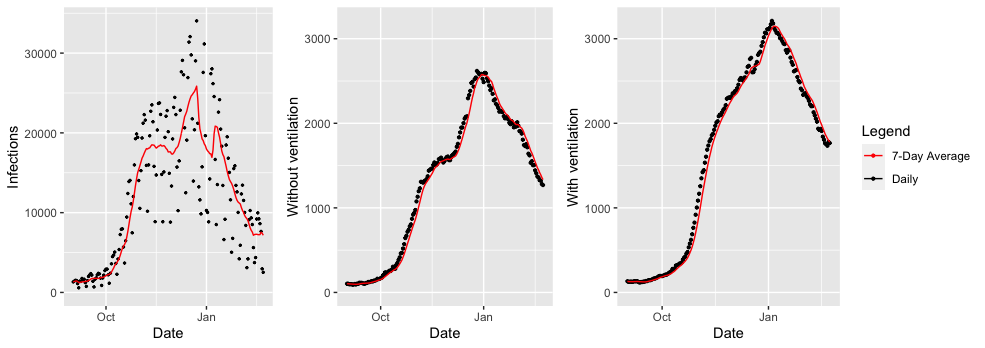
\includegraphics[width=0.97\linewidth]{rkiDiviData.png}
    \caption{Visualization of current German COVID-19 Data as used in \babsimhospital. From left to right: Daily new infections as published by the Robert-Koch Institute, amount of occupied intensive care beds in hospitals (without invasive ventilation), amount of invasively ventilated intensive care beds.}
\label{fig:rki}
\end{figure*}
\gls{ETL} processes integrate data from various sources into complex collections~\cite{ELSAPPAGH201191}. 
After the successful extraction of data, the next step is to transform it. 
This step includes several approaches to gain accurate data which is correct, complete, consistent, and unambiguous.  
The final step consists of loading the processed data into a data collection of choice accessible for the data analyst for further use.
Especially in terms of the COVID-19 pandemic, it is important to integrate and process the vast amount of constantly growing data. 

\subsubsection{Germany}
The on-line version of the \babsimhospital simulator implements an \gls{ETL} process to analyze the data from the \gls{RKI}, \url{https://www.rki.de}, as well as the \gls{DIVI}, \url{https://www.divi.de}.
The associated data sets contain anonymous information about every recorded case in Germany. The \gls{RKI} data set contains 
780,065 observations of 18 variables such as age, gender, data of infection, etc., which were updated daily and are automatically integrated into \babsimhospital. 
Information concerning \gls{ICU} in Germany can be retrieved from the \gls{DIVI}.
\gls{DIVI} provides an API and a daily report. 
The official simulator, which can be accessed via \url{https://www.th-koeln.de/babsimhospital}, uses \gls{DIVI} and \gls{RKI} data.
Its parameters are based on discussions with experts from Germany, especially \gls{ICU} doctors and experts from health administration.
The online version is described in Section~\ref{sec:online}.



\subsubsection{UK}
\begin{figure*}
    \centering
    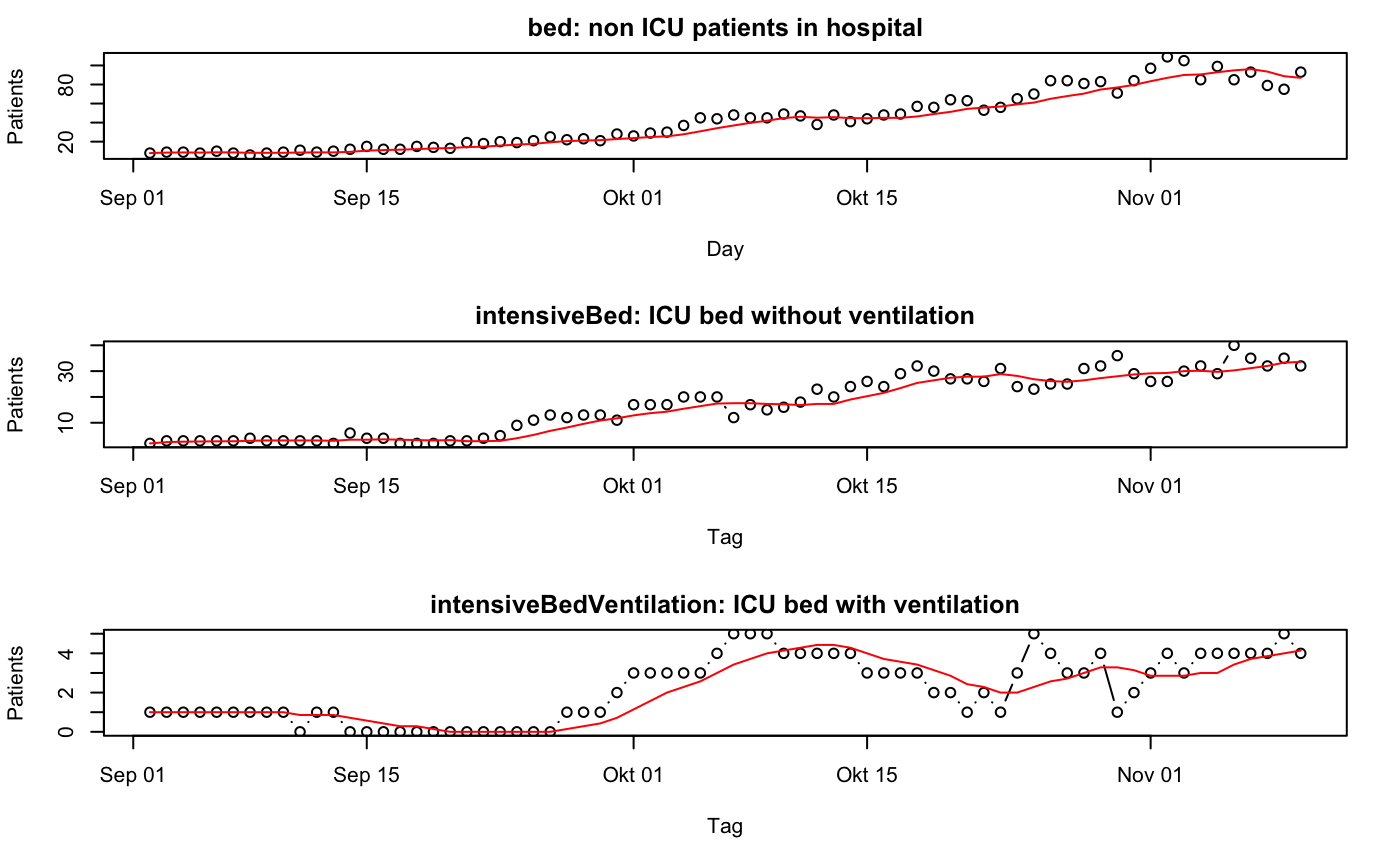
\includegraphics[width=0.75\linewidth]{ukdata3.png}
    \caption{UK data. Dots denote real-world data, red lines represent the seven-day average. \gls{ICU} beds with ventilation are shown in the last row. The UK has far fewer \gls{ICU} ventilator beds than Germany.}
\label{fig:ukdata}
\end{figure*}

This paper describes an extension of the interface that enables usage of data independently from \gls{DIVI} and \gls{RKI} data, i.e., an interface to \gls{CSV} files and Excel files can be used so that any kind of field and simulation data can be processed, simulated, and optimized.
To exemplify our approach, anonymised data from a region in the UK was used. 
The data was read from an Excel file, which has the following entries (columns):
\begin{compactitem}
\item date
\item bed: total number of patients in hospital with \gls{COVID-19} (includes \gls{ICU})
\item intensiveBed: number of patients on non-invasive ventilators (CPAP). In normal circumstances they would be on \gls{ICU} or equivalent but in the UK this has not always been possible.
\item intensiveBedVentilation: number of patients intubated and ventilated with \gls{COVID-19} on \gls{ICU}
\end{compactitem}
The field data based on UK data used three bed categories: 
\begin{compactenum}
\item bed: non ICU patients in hospital
\item intensiveBed: ICU bed without ventilation
\item intensiveBedVentilation: \gls{ICU} bed with ventilation
\end{compactenum}
\figref{fig:ukdata} visualizes the UK data set that is used in this study. The whole data set consists of data from 240 days. Since our analysis considers the second \gls{COVID-19} wave only, we use data after September 2020.

\section{The Simulator}\label{sec:sim}
\subsection{Discrete Event Simulation}
\babsimhospital simulates the typical paths that COVID-19 infected patients follow during their hospital stays. 
The \gls{DES} processes every single recorded infection until the patients' recovery or death. 
Patients follow a trajectory, i.e., they move with a probability $p_{ij}$ from state $S_i$ to state $S_j$  after a transition-specific duration $d_{ij}$.
Parameter settings consist of
\begin{compactitem}
\item transition probabilities, e.g., the probability that an infected
   individual has to go to the hospital. 
\item  durations, e.g., the time span until an infected individual goes to the
   hospital (in days). 
\end{compactitem}
A graph can be used to model this behavior.
\figref{fig:prob} illustrates the transition probabilities and describes the states.

\begin{figure}
    \centering
    %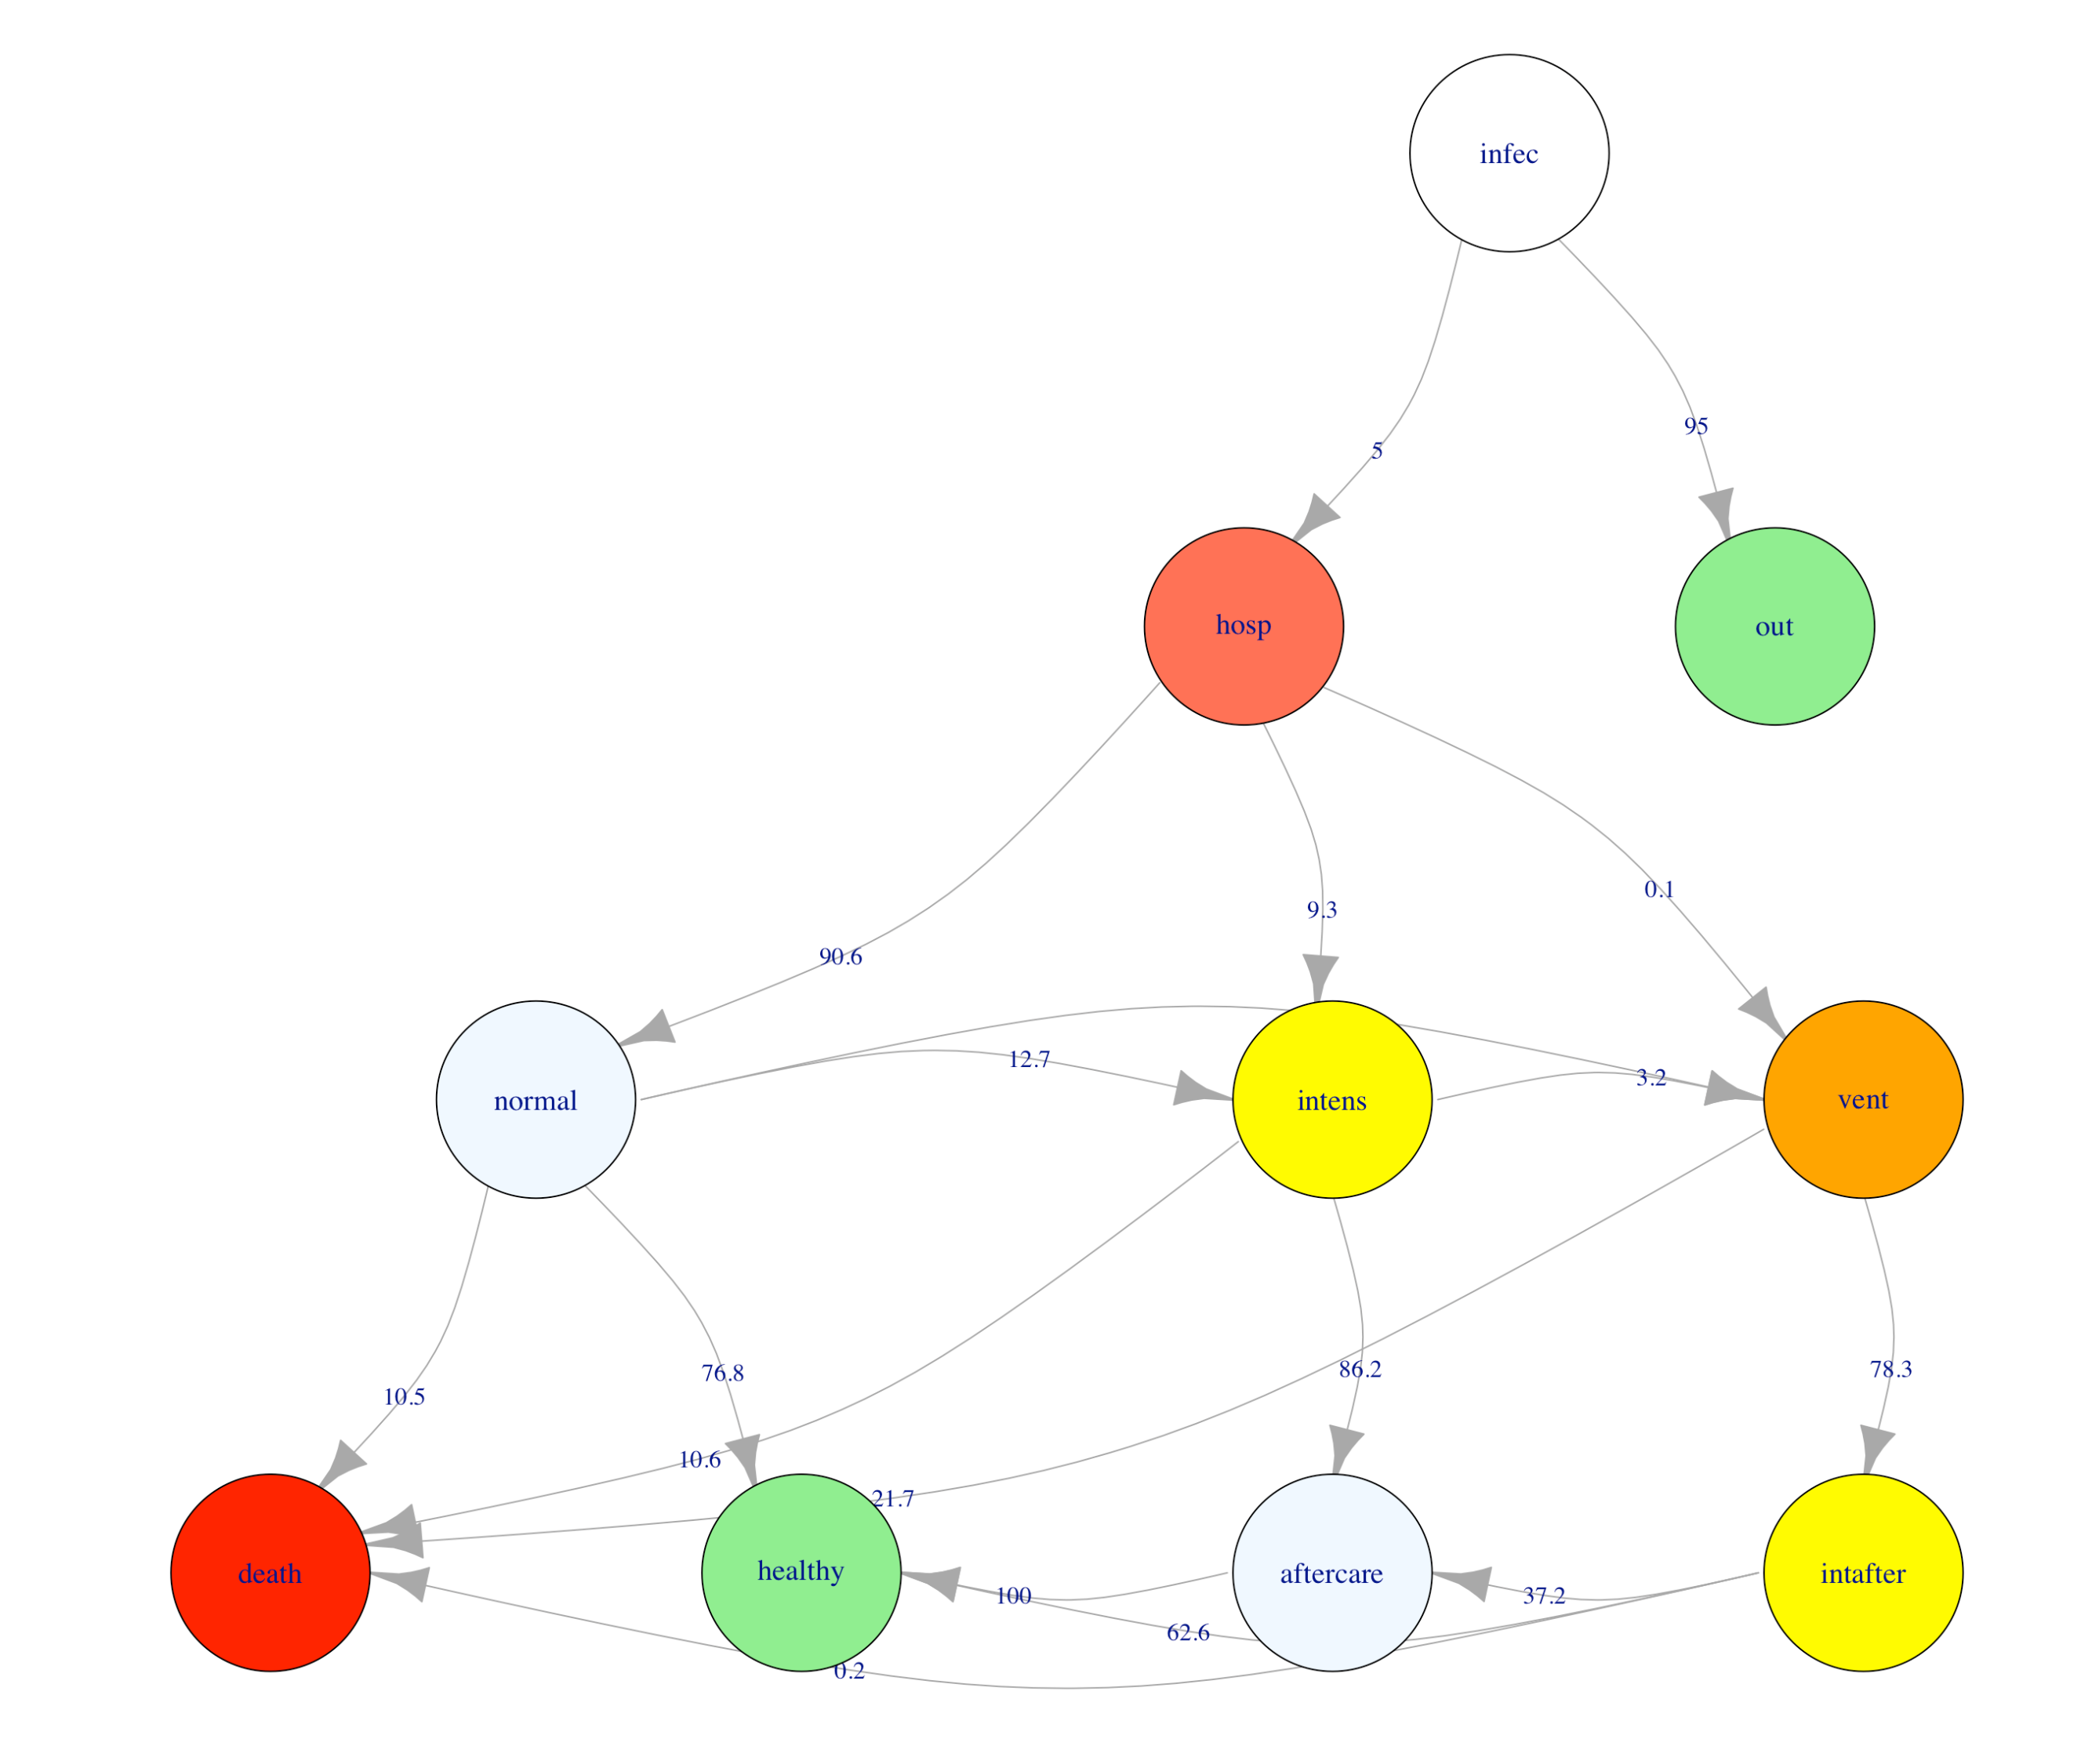
\includegraphics[width=0.75\linewidth]{prob.png}
    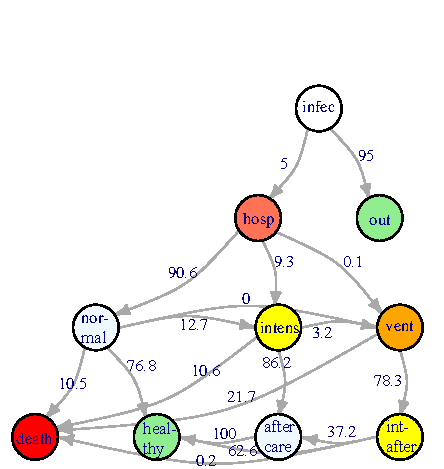
\includegraphics[width=\linewidth]{modelgraph.pdf}
    \caption{Full model of patient flows in a hospital. Nodes represent states ($S_i$). Edges represent state changes with associated probabilities ($p_{ij}$). The nodes are labeled as follows: \emph{Infec:}\/ Number of people tested positive for Covid-19, published by RKI, 
\emph{out:}\/ Infected people not hospitalized, \emph{hosp:}\/ Hospitalized infected people, \emph{normal:}\/ Isolation ward, \emph{intens:}\/ Intensive care ward without invasive ventilation, \emph{vent:}\/ Intensive care ward with invasive ventilation, \emph{intafter:}\/ Intensive aftercare ward without invasive ventilation, \emph{aftercare:}\/ Aftercare isolation ward, \emph{healthy:}\/ Discharged as recovered, and \emph{death:}\/ Deceased.
This graph shows the core of \babsimhospital. This sets \babsimhospital apart from other simulators. It enables a detailed analysis of the underlying events. Upon request, it can be adapted to the individual circumstances of interested parties.}
\label{fig:prob}
\end{figure}

For example, an infected patient (state $S_1$) goes to the hospital (state $S_2$) with probability $p_{12}$ after $d_{12}$ days. With probability $p_{17}$, she recovers (state $S_7$) after $d_{17}$ days. 
The probabilities of outgoing nodes sum to 1, e.g., $p_{17} = 1 - p_{12}$.
The modeling process includes four types of parameters: 
\begin{description}
\item[transition probabilities,] e.g., the probability that an infected individual has to go to the hospital,
\item[durations,] e.g., the time span until an infected individual goes to the hospital (in days), and
\item[distribution properties,] e.g., truncated and translated gamma distribution,
\item[risk factors] depending on demographic groups, e.g., age, gender. 
\end{description}
The on-line version of the \babsimhospital simulator uses risk information: every new patient is assigned a unique risk. 
Although the "risk" attribute is an important factor for the duration and severity of a \gls{COVID-19} infection, it was not considered in our study. However, it can easily be integrated in future studies. 
Table~\ref{tab:para} presents an overview of the parameter ranges of the 29 parameters used in the \babsimhospital simulation model.

% latex table generated in R 4.0.4 by xtable 1.8-4 package
% Tue Feb 23 15:02:12 2021
\begin{table*}[ht]\label{tab:para}
\caption{Default (DE) and adapted (UK) ranges of the 29 parameters. Parameters that were  modified for the UK setting are shown in \textbf{bold face}. The prefix \emph{AmntDays*}\/ refers to durations (in days), whereas the prefix \emph{FactorPatients*}\/ refers to proportions/probabilities. The column \emph{default} shows recommendations from experts in Germany, \emph{minUK} and \emph{maxUK} denote adapted ranges from the UK, and \emph{minDE} and \emph{maxDE} represent the parameter ranges from Germany.}  
\centering
\begin{tabular}{llrrrrr}
  \hline
Variable & Name & default & minUK & maxUK & minDE & MaxDE \\ 
  \hline
$x_1$&  AmntDaysInfectedToHospital & 9.5 &   6 &  14 &   6 &  14 \\
$x_2$&   AmntDaysNormalToHealthy&  10 &   7 &  13 &   7 &  13 \\
$x_3$&   AmntDaysNormalToIntensive &   5 &   3 &   7 &   3 &   7 \\ 
$x_4$&  AmntDaysNormalToVentilation & 3.6 &   3 &   9 &   3 &   9 \\ 
$x_5$&   AmntDaysNormalToDeath&   5 &   3 &   7 &   3 &   7 \\  
$ \mathbf{x_6}$&   \textbf{AmntDaysIntensiveToAftercare} & $\mathbf{7}$ & $\mathbf{10}$ & $\mathbf{18}$ & $\mathbf{5}$ & $\mathbf{9}$ \\ 
$\mathbf{x_7}$ &   \textbf{AmntDaysIntensiveToVentilation} & $\mathbf{4}$ & $\mathbf{6}$ & $\mathbf{10}$ & $\mathbf{3}$ & $\mathbf{5}$ \\ 
$\mathbf{x_8}$&   \textbf{AmntDaysIntensiveToDeath} & $\mathbf{5}$ & $\mathbf{6}$ & $\mathbf{14}$ & $\mathbf{3}$  & $\mathbf{7}$ \\ 
$x_9$&   AmntDaysVentilationToIntensiveAfter &  30 &  25 &  35 &  25 &  35 \\ 
$x_{10}$&   AmntDaysVentilationToDeath  &  20 &  17 &  25 &  17 &  25 \\  
$x_{11}$&   AmntDaysIntensiveAfterToAftercare &   3 &   2 &   5 &   2 &   5 \\ 
$x_{12}$&   AmntDaysIntensiveAfterToDeath &   4 &   1 &   7 &   1 &   7 \\ 
$x_{13}$&   GammaShapeParameter &   1 & 0.25 &   2 & 0.25 &   2 \\ 
$x_{14}$&   FactorPatientsInfectedToHospital & 0.1 & 0.05 & 0.15 & 0.05 & 0.15 \\ 
$x_{15}$&   FactorPatientsHospitalToIntensive & 0.09 & 0.07 & 0.11 & 0.07 & 0.11 \\ 
$ \mathbf{x_{16}}$ & \textbf{FactorPatientsHospitalToVentilation} & $ \mathbf{0.01}$ & $ \mathbf{0.001}$ & $ \mathbf{0.004} $& $ \mathbf{0.005}$ & $ \mathbf{0.02}$ \\ 
$x_{17}$&   FactorPatientsNormalToIntensive & 0.1 & 0.07 & 0.13 & 0.07 & 0.13 \\ 
$\mathbf{x_{18}}$&   \textbf{FactorPatientsNormalToVentilation} & $\mathbf{0.001}$ & $\mathbf{2e-05}$ & $\mathbf{0.0004}$ & $\mathbf{0.0001}$ & $\mathbf{ 0.002}$ \\ 
$x_{19}$&   FactorPatientsNormalToDeath & 0.1 & 0.08 & 0.12 & 0.08 & 0.12 \\ 
$\mathbf{x_{20}}$&   \textbf{FactorPatientsIntensiveToVentilation} & $\mathbf{0.3}$ & $\mathbf{0.05}$ & $\mathbf{0.07}$ & $\mathbf{0.25}$ & $\mathbf{0.35}$ \\ 
$x_{21}$&   FactorPatientsIntensiveToDeath & 0.1 & 0.08 & 0.12 & 0.08 & 0.12 \\  
$x_{22}$&   FactorPatientsVentilationToIntensiveAfter & 0.7 & 0.5 & 0.9 & 0.5 & 0.9 \\ 
$x_{23}$&   FactorPatientsIntensiveAfterToDeath & 1e-05 & 1e-06 & 0.01 & 1e-06 & 0.01 \\ 
$x_{24}$&   AmntDaysAftercareToHealthy &   3 &   2 &   4 &   2 &   4 \\ 
$x_{25}$&   RiskFactorA & 0.02 & 1e-06 & 1.1 & 1e-06 & 1.1 \\
$x_{26}$&   RiskFactorB & 0.01 & 1e-06 & 0.062 & 1e-06 & 0.062 \\ 
$x_{27}$&   RiskMale & 1.5 &   1 &   2 &   1 &   2 \\  
$x_{28}$&   AmntDaysIntensiveAfterToHealthy &   3 &   2 &   5 &   2 &   5 \\ 
$x_{29}$&   FactorPatientsIntensiveAfterToHealthy & 0.67 & 0.5 & 0.75 & 0.5 & 0.75 \\ 
   \hline
\end{tabular}
\end{table*}

Proper tuning of these parameters is essential to obtain accurate predictions based on up-to-date and local data. 
The time-dependent changes require a frequent refitting of the model parameters to the current situation.
Thus, a daily parameter tuning procedure is run for each German region in order to provide an accurate prediction.
An initial estimate for each of the given parameters was specified in cooperation with medical professionals. 
For example, the rate of successful treatments in Germany drastically changed between the first and the second wave of COVID-19 infections. 
Also, political decisions on national and local level can affect the situation significantly. 
While reducing the access to nursing homes might reduce infections in the high risk parts of the population, opening schools might cause many infections in the younger parts of the population. The optimization problem can be stated as follows:
the \babsimhospital simulator requires two input parameters (vectors), $\vec{x}_t$, the model parameters, and $\vec{u}_t$, the number of infections. Based on these two inputs, \babsimhospital estimates the required resources---in our case, the beds, \gls{ICU} beds,  and \gls{ICU} beds with ventilators.
The simulation output, i.e, the required resources on each day $t$ will be denoted as $\hat{\vec{y}}_t$, i.e., 
\begin{equation}\label{eq:haty}
\hat{y}_t = \left( \hat{R}_{\text{bed}}(t),   \hat{R}_{\text{icu}}(t), \hat{R}_{\text{vent}}(t) \right)
\end{equation}
The \gls{DES} delivers valid results and enables predictions, which are valuable for capacity planning in hospitals.
The \gls{simmer} software presents a good basis for implementation and was able to handle more than half a million data (infections) under very limited time constraints. 

\subsection{The Online-Version}\label{sec:online}
%%% TODO: Besser formulieren, mit Abbildung verknuepfen
An online version of \babsimhospital, 
which includes a graphical user interface, 
makes the simulator available and accessible to the public, see \url{https://covid-resource-sim.th-koeln.de/app/babsim.hospitalvis}.
\figref{fig:demo} shows a screenshot of this application.
\begin{figure*}
    \centering
    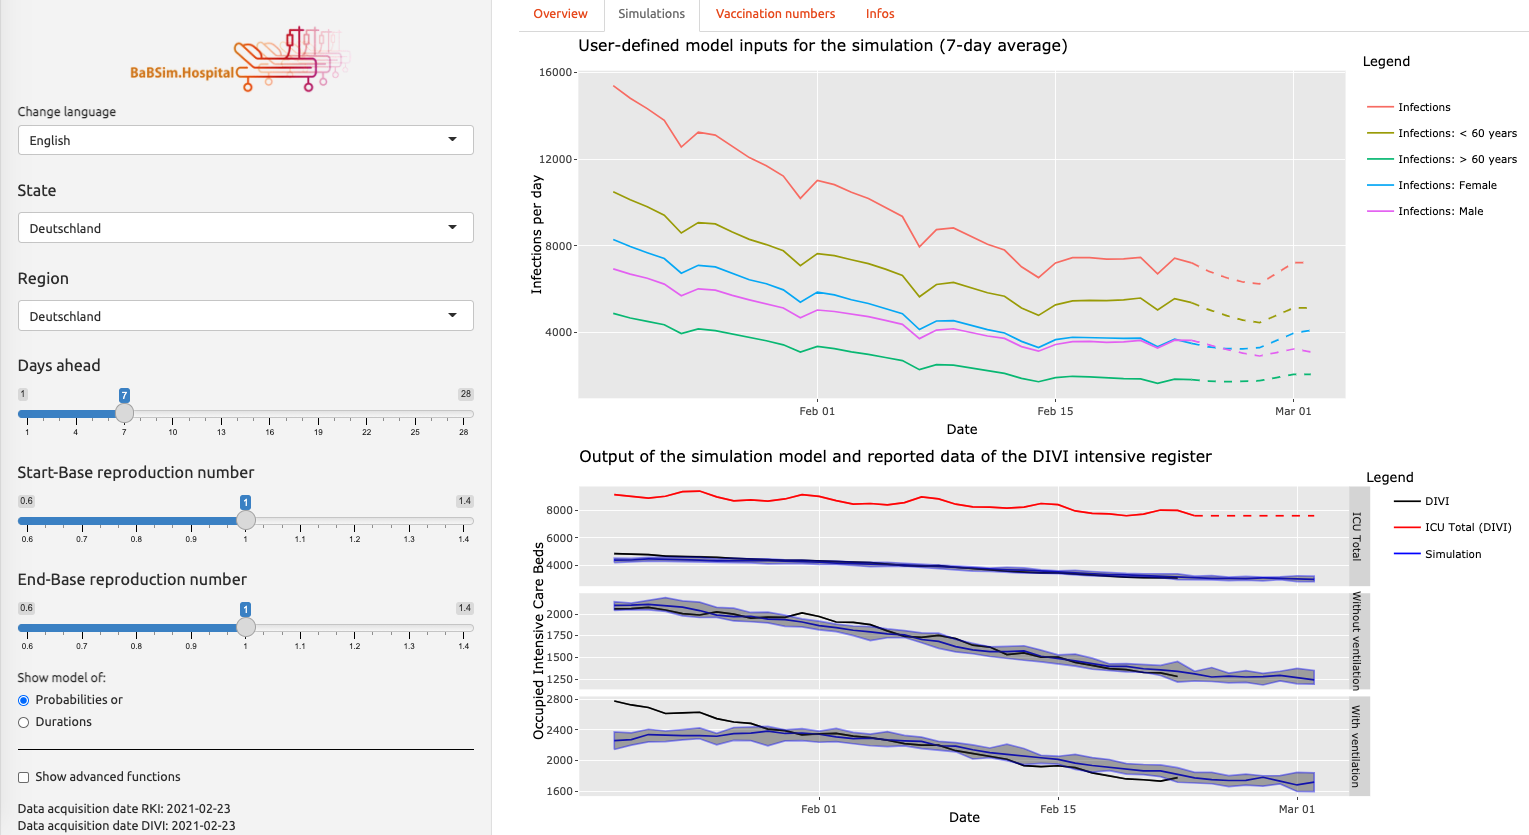
\includegraphics[width=\linewidth]{demoFR.png}
    \caption{Online version. Users are able to select different countries and regions to simulate
for, as well as some very general configurations (time window for
the simulation, assumptions about the virus' reproduction factors, as well as some choices of different visualizations).}
\label{fig:demo}
\end{figure*}
%The application has the following advantages for crisis teams:
%\begin{compactitem}
%\item Comparison of the simulation results with their own data and planning tools.
%\item Simulation based on local/regional events and circumstances.
%\item Simulation of different worst or best-case scenarios (w.r.t. reproduction numbers).
%\item Standardized approach to simulation and visualization of the results.
%\end{compactitem}
%It provides benefits for medical professionals, e.g.,
%\begin{compactitem}
%\item Analysis of the pandemic's impact at local, regional, state and federal level.
%\item Consideration of special risk groups.
%\item Validation of the length of hospital stays.
%\item Validation of the probabilities.
%\end{compactitem}
%Lastly, administration and management can
%\begin{compactitem}
%\item assess of the situation at individual hospitals taking local events into account,
%\item consider relevant resources: beds, ventilators, rooms, protective clothing,
%\item and perform personnel planning (medical and nursing staff).
%\end{compactitem}

%\subsection{Open Source}
\babsimhospital is open source. It is programmed in the R programming language and freely available, see~\cite{bart20t}.
The online-version is running fully automatically for several months.
It allows processing  the \gls{RKI} data set, which consists of more than 
750,000 observations of 18 variables, which are updated daily and are automatically integrated into \babsimhospital simulator. 
The \gls{CICD} approach minimizes human interaction, so that simulations and optimizations are
started automatically after the data is downloaded.

\section{Optimization}\label{sec:optim}
Based on the simulation results, optimization runs can be performed to improve parameter settings proposed by the experts. 
The \gls{RMSE} as shown in Eq.~\ref{eq:rmse}, is used to measure the error of the simulator.
We formulate the \emph{minimization} problem:
\begin{equation}\label{eq:rmse}
  \min 
  \sum_{k\in\{\text{bed},\text{icu},\text{vent}\}}
    w_k  \sqrt{\frac{1}{T} \sum_{t=1}^T \left(R_k(t) - \hat{R}_k(t)\right)^2}
\end{equation}
Here, $T$ denotes the number of days simulated and $k$ the three different bed categories.
Since the different bed types are not equally important a weighted average of the \gls{RMSE} for each bed category is used as the final error measure.
A detailed description can be found in~\cite{Bart20j}.

The extensive amount of data that the tool has to process combined with the high dimension of the problem, and the required accuracy make simplifying the modeling process to improve performance a big challenge.
The limited time available for each optimization run requires the use of efficient algorithms.

The following state-of-the-art optimization approaches were considered: 
\begin{compactitem}
\item stand-alone, standard optimization algorithms, e.g., BOBYQA~\cite{Powe09a}, CMA-ES~\cite{Hans06a}, Simulated Annealing~\cite{vanL87a},
\item response surface methodology and surrogate model-based optimizers~\cite{Myers2016}, 
\item parallelized  combinations of global with local optimizers~\cite{Good18b},  
\item massively parallel single-iteration optimizers~\cite{Cauw20a,Rena20a}, and 
\item \gls{SMBO} approaches~\cite{Jin11a}.
\end{compactitem}
First, the applicability of these different approaches  was tested. Pre-experimental results revealed that only \gls{SMBO} approaches produced good results. 
Therefore, the \gls{SPOT} algorithm was chosen~\cite{Bart17parxiv}.
To accelerate the \gls{SPOT}, simulations were run in parallel. 

\section{Adaptation of the Search Boundaries}\label{sec:adaptation}

\begin{figure*}[t]
  \centering
   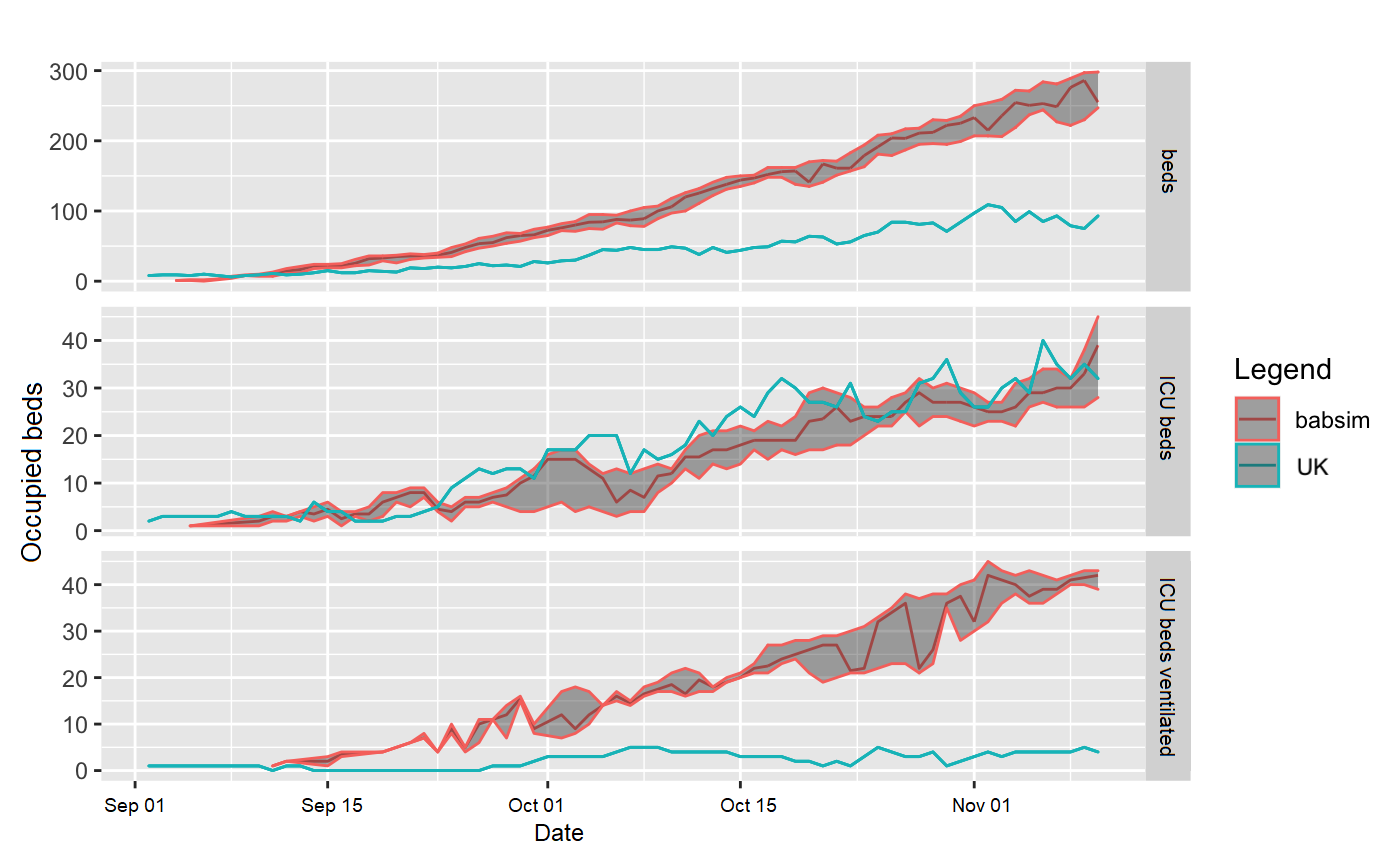
\includegraphics[width=0.49\textwidth]{default.png}
    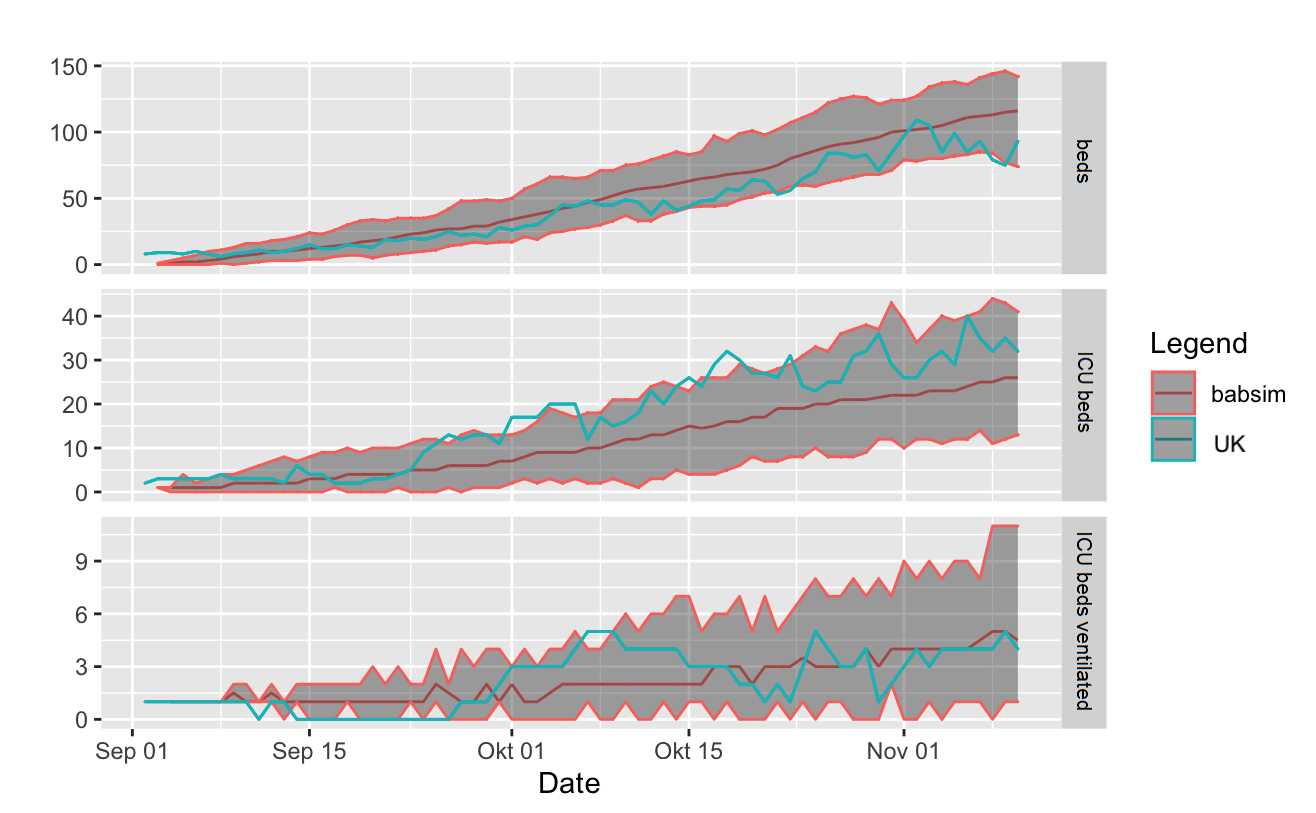
\includegraphics[width=0.49\textwidth]{optimzed01b.png}
  \caption{\emph{Left:}\/ Real data compared to results from the \babsimhospital simulation with default parameters. Large residuals (errors), especially for normal bed and ICU beds with ventilation can be observed.
   \babsimhospital uses default parameter sets. These are based on domain knowledge (recommendations from doctors) from Germany. \emph{Right:}\/ Real data compared to results from the \babsimhospital simulation with optimized parameters. The  $c_1$ value was set to $0.2$. Considering the regular \gls{ICU} beds (category II) there is still a difference between the real data from the UK and the simulated data. Therefore, a second adaption was necessary. }
\label{fig:default}
\end{figure*}
\begin{figure}[t]
    \centering
    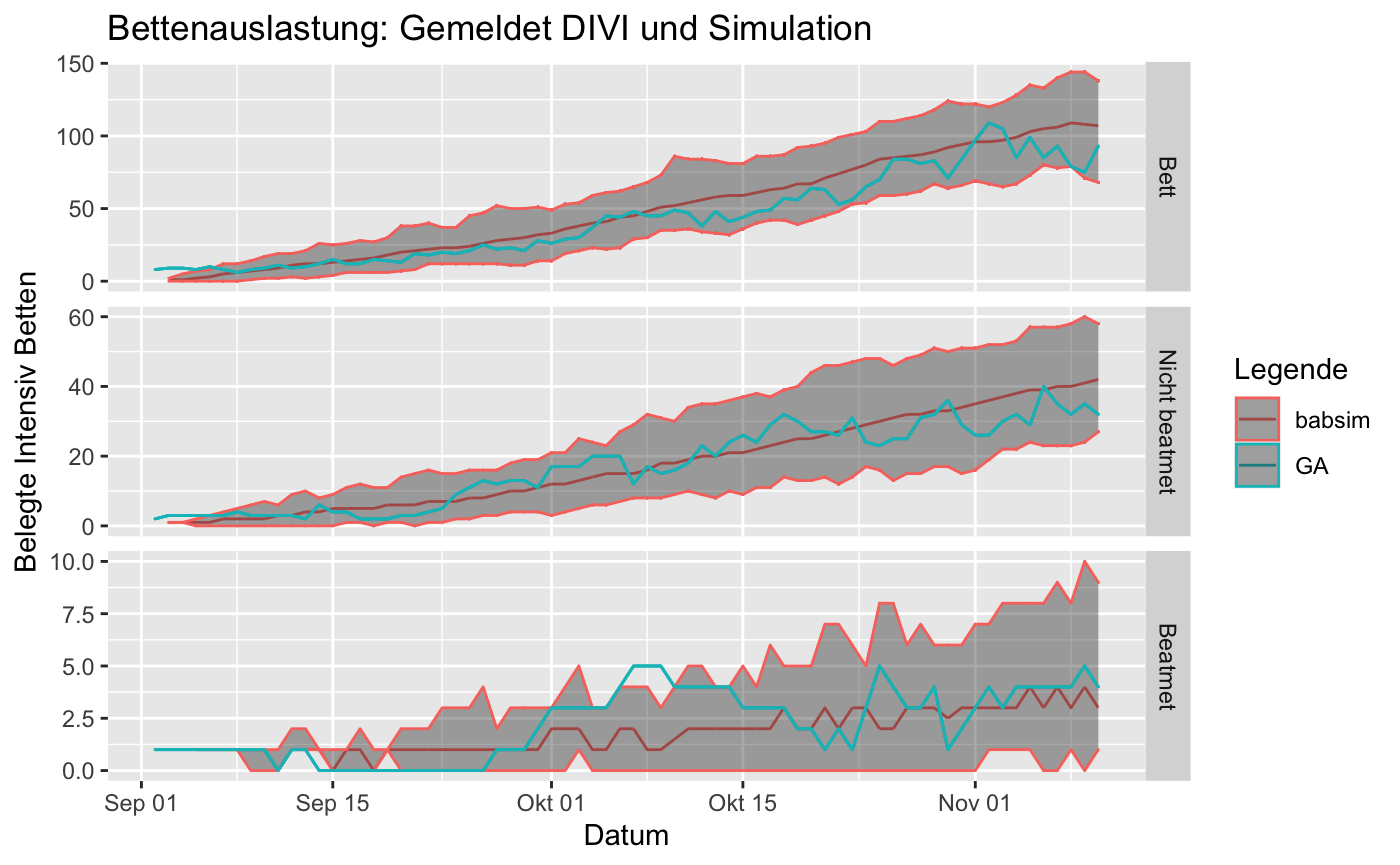
\includegraphics[width=0.49\textwidth]{optimized02.png}
    \caption{Real data compared to results from the \babsimhospital simulation with optimized parameters. The comparison with the results from Fig.~\ref{fig:default} shows a significant improvement. Residuals are much smaller,
    because the simulation model parameters were adapted to the situation in UK hospitals. Additionally, simulation results for category II beds is improved.  
  }
\label{fig:optimized02}
\end{figure}


The UK has markedly fewer ICU beds than Germany (6.6 per 100,000 versus 29.2 per 100,000 in 2011  \cite{rhodes_variability_2012}).
Therefore, patients may be treated differently: the clinical threshold for a patient to be admitted to ICU may be higher than in Germany. We can adapt the boundaries of the search space (constraints) to reduce the probability of a patient being sent to \gls{ICU}.

\subsubsection{First Adaptation---Reducing Probabilities}
To implement the different setting, we modified the parameter boundaries (see Table~\ref{tab:para}) as follows: vent, i.e, the \gls{ICU} with ventilation node that is colored in orange in \figref{fig:prob}) has three incoming edges: from node normal, node hosp, and node intens.
By introducing a reduction factor, say  $c_1 \in \mathbb{R_+}$, that simply multiplies the default probabilities of patients reaching the ICU ventilated node, we were able to redirect patients to other bed categories. Because the sum  of the probabilities of the outgoing edges must be $1.0$, the modification of one probability also changes the probabilities of the associated edges in the model (see \figref{fig:prob}).
Choosing a value of $c_1=0.2$ results in improved simulation outputs, and plausibly reflects real-world differences in the provision of ICU beds in the UK compared to Germany. Please note that $c_1$ does not directly affect the probabilities, it modifies the search boundaries (constraints) of the optimizer.

The range of the parameter 
$x_{16}$ that describes the proportion of patients that go directly to ICU with ventilation 
was reduced from $[0.01; 0.02]$ to $[5.0e-04; 0.004]$. In addition, the range of the parameter $x_{18}$, which represents the proportion of patients that go from normal beds to ICU with ventilation was reduced from $[0.1; 0.2]$ to $[0.02; 0.04]$. Furthermore, 
the range of parameter $x_{20}$ that describes the proportion of patients that go from ICU to ICU with ventilation was reduced from $[0.1; 0.2]$ to $[0.02; 0.04]$. 

As a consequence of the reduced search intervals of $x_{16}$, $x_{18}$, and $x_{20}$, simulation results of the ventilated \gls{ICU} beds were significantly improved.: the numerical \gls{RMSE} goes down from $184.10$ to $46.94$. This improvement is also validates by visual inspection as can be seen in the \emph{right} panel of \figref{fig:default}.

\subsubsection{Second Adaptation---Increasing Durations}

However, even if the ventilated ICU bed usage was improved (bed category III), the simulation of the second bed category is not satisfying. We under estimate the number of ICU beds. This may be a result of the higher UK threshold for ICU admission meaning that the average UK ICU patient is more unwell than the average ICU patient in Germany. To fix this problem, we modified the duration of patients in ICU beds: the search intervals of these parameters were increased. Therefore, a second factor, say $c_2 \in \mathbb{R}_+$ was introduced to multiply the corresponding durations. A value of $c_2 = 2.0$ was chosen for our experiments.
The range of the parameter  $x_{6}$ that represents the number of days  patients stay at ICU with ventilation before they go to intensive aftercare was increased from $[5;9]$ to $[10;18]$ days. The range of the
parameter $x_{7}$  that defines the  number of days before ICU  patients go to ICU with ventilation was increased from $[3;5]$ to $[6;10]$ days. Finally, the interval of the parameter $x_{8}$, which specifies the number of days patients stay at ICU before they die, was increased from $[3;7]$ to $[6;14]$ days.


\section{Results}\label{sec:results}


The adaptation of the parameter bounds based on domain knowledge results in a significant reduction of the \gls{RMSE}, which was defined in  Eq.~\ref{eq:rmse}. 
Using the default \babsimhospital parameter boundaries, which were based on the situation in Germany, the simulation error is $\epsilon_0 = 184.10$.
The first adaptation, which reduces the percentage of patients treated in \gls{ICU} beds with ventilation, results in an simulation error $\epsilon_1 =  46.94$, whereas the second adaption, which increases the time patients spend in an \gls{ICU} bed results in a further reduction of the simulation error to $\epsilon_2 = 29.0$. In summary, the adaptation has been shown to reduce simulation errors by nearly 70\%.
Figures~\ref{fig:default} and \ref{fig:optimized02} clearly visualize the improvements.


\section{Discussion and Outlook}\label{sec:discussion}
The \babsimhospital simulator, an open-source tool for capacity planning based on discrete event simulation,  was developed over the last year to support doctors, administrations, health authorities, and crisis teams in Germany.
The high dimension and computational expense of the \babsimhospital simulator 
poses a challenging optimization task. 
Solving this task for many regions in Germany under very different local circumstances requires 
efficient solutions to cope with the further growing infection numbers and thus also growing simulation run times. 
A \gls{SMBO} approach delivers stable and valid results for every state and region in Germany.

Estimating the effort of transferring the simulator to different regions is of great interest. 
Based on data from the UK, we demonstrated that an adaption of the search ranges (bound constraints) of the associated optimizer leads to satisfactory results. 

The questions posed in Section~\ref{sec:intro} can be answered as follows:
\begin{compactenum}[(Q-1)]
\item The extended version of the \babsimhospital interface is able to process any input data that contains information about the date, the number of beds (this information is optional), the number of patients on non-invasive ventilation, and the number of patients intubated and ventilated. Using real-world data from the UK, we successfully demonstrated how these data can be processed by the simulator.
The adaption from the German health-care system to the UK system can be achieved by changing the search ranges of the optimizer----and not the absolute parameter values of the simulator. This modification of these ranges is much more easier than the modification of specific values, because ranges are easier to specify than point values. Interestingly, the same factor as the relative number of \gls{ICU} beds ($c_1$ was chosen as $1/5$, which reflects the difference in the number of \gls{ICU} beds in the UK versus Germany~\cite{rhodes_variability_2012}) was useful for the first adaptation (as even $c_1=1/5 $ seems extreme until you know how different the two countries are!).
Our study reveals that simulations with \babsimhospital are not restricted to the health system in Germany.
\item This study clearly demonstrates that domain knowledge is essential for obtaining reliable and valid simulation results. Especially in high dimensional search spaces, optimizers can deliver results that are mathematically optimal, but practically irrelevant. The discussion delivers important insights into the problem. 
\end{compactenum}
Furthermore, the \babsimhospital simulator can be used as attractive simulation and optimization benchmark example. Its source code is open source. 
Knowing the optimiser's output in terms of number of days for each transition in the model, and their probability, is interesting to clinicians. Plausibly it could help compare treatment strategies where hospitals have acted differently. For example, some hospitals used a lot of \gls{CPAP} but other centres used less and therefore had to move earlier to ventilation.
One particular advantage of modelling in the UK has been estimating how much spare capacity there is in hospitals for continuing elective surgery such as arranging cancer operations etc.

\section*{Reproducibility}
The programming code as well as the data, which was used in this study, will be published on CRAN as a vignette of the next version of the R  package \babsimhospital, see \url{https://CRAN.R-project.org/package=babsim.hospital}.  

\section*{Acknowledgment}
T.~Bartz-Beielstein acknowledges support from the \emph{Ministerium f{\"u}r Kultur und Wissenschaft des Landes Nordrhein-Westfalen}\/ in the funding program \emph{FH Zeit f{\"u}r Forschung}\/ under the grant number 005-1703-0011 (project OWOS) and support from the \emph{German Federal Ministry of Education and Research}\/ in the funding program \emph{Forschung an Fachhochschulen}\/ under the grant number 13FH007IB6 (project KOARCH). 



%% TODO: finally, we have to change this and use simple brackets :-( 
%\bibliographystyle{ACM-Reference-Format}
\bibliographystyle{IEEEtran}

\bibliography{sample-base}
\end{document}
\endinput

